\begin{remark}
    На прошедшей конференции KDD 2020 30\% всех статей было посвящяно Graph ML, так что это определенно область, к которой стоит присмотреться повнимательнее. 
\end{remark}

Статья\footnote{\url{https://towardsdatascience.com/top-trends-of-graph-machine-learning-in-2020-1194175351a3}} про интересные приложения Graph ML, в том числе для построения рекомендаций.

\section{[Google] Unsupervised Graph Representations}

\textbf{Video:}~\url{https://youtu.be/J3h_15iu4gE} \\

Обзорный доклад посвященный большому числу работ по обучению embedding'ов вершин графов.

В докладе излошены основные идеи методов.

\begin{figure}[ht]
    \centering
    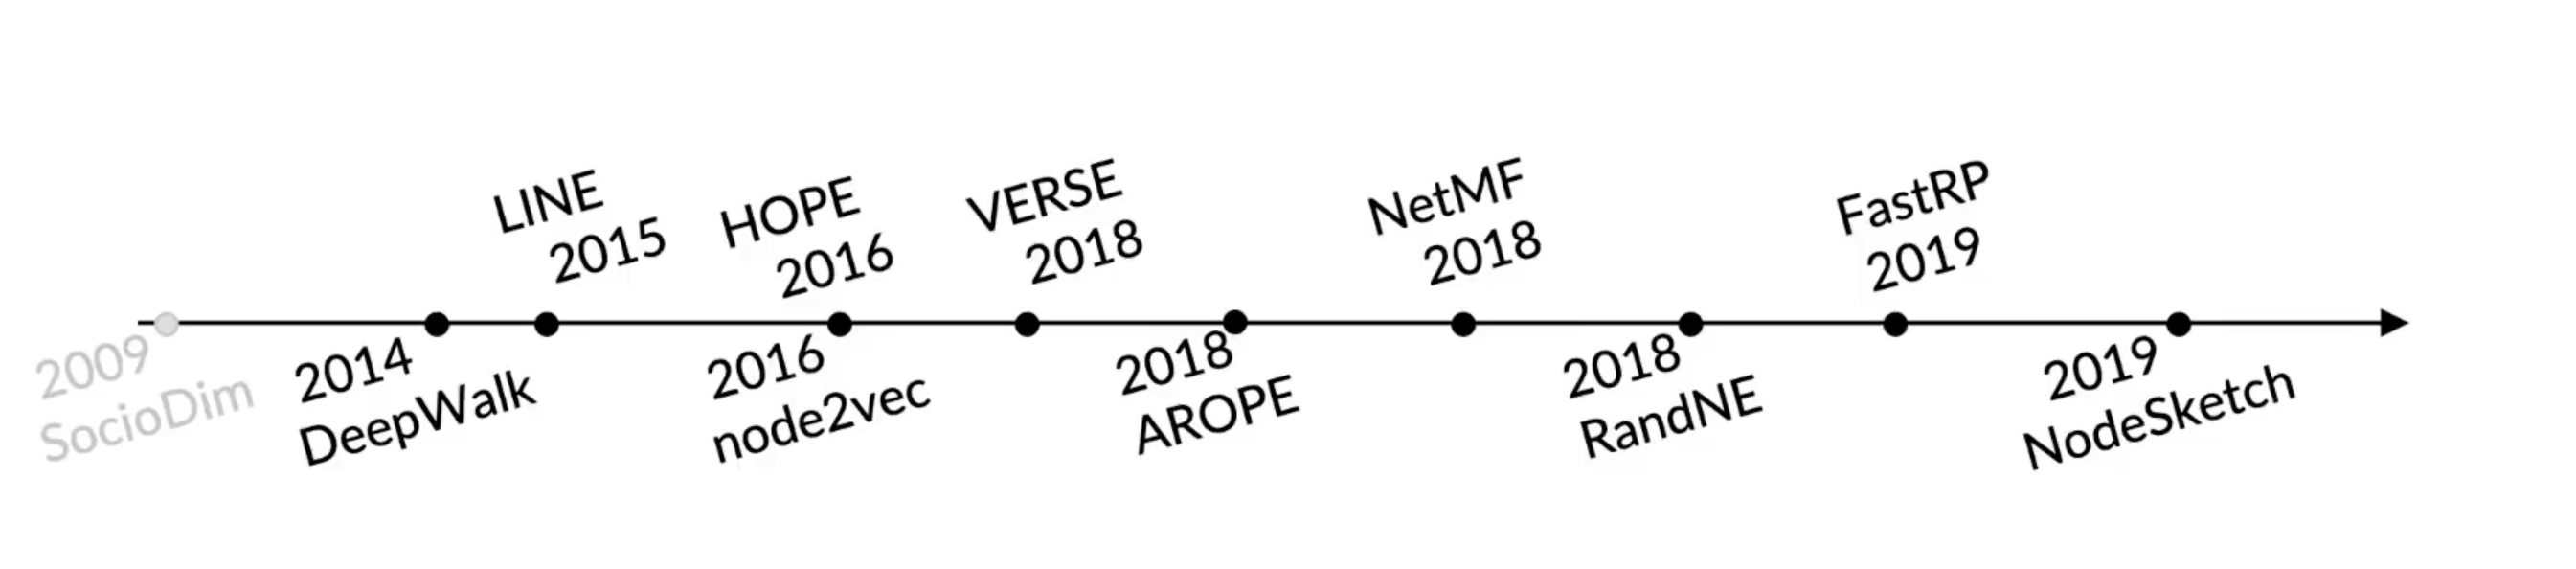
\includegraphics[width=0.9\linewidth]{images/graph_emb.png}
\end{figure}

\section{[Skoltech] Link Prediction with Graph Neural Networks}

\textbf{Video:}~\url{https://youtu.be/WNQi_kvdlr4} \\

Еще один обзорный доклад посвященный задаче предсказания ребер с помощью графовых нейросетей.